% Created by tikzDevice version 0.9 on 2015-12-14 00:25:55
% !TEX encoding = UTF-8 Unicode
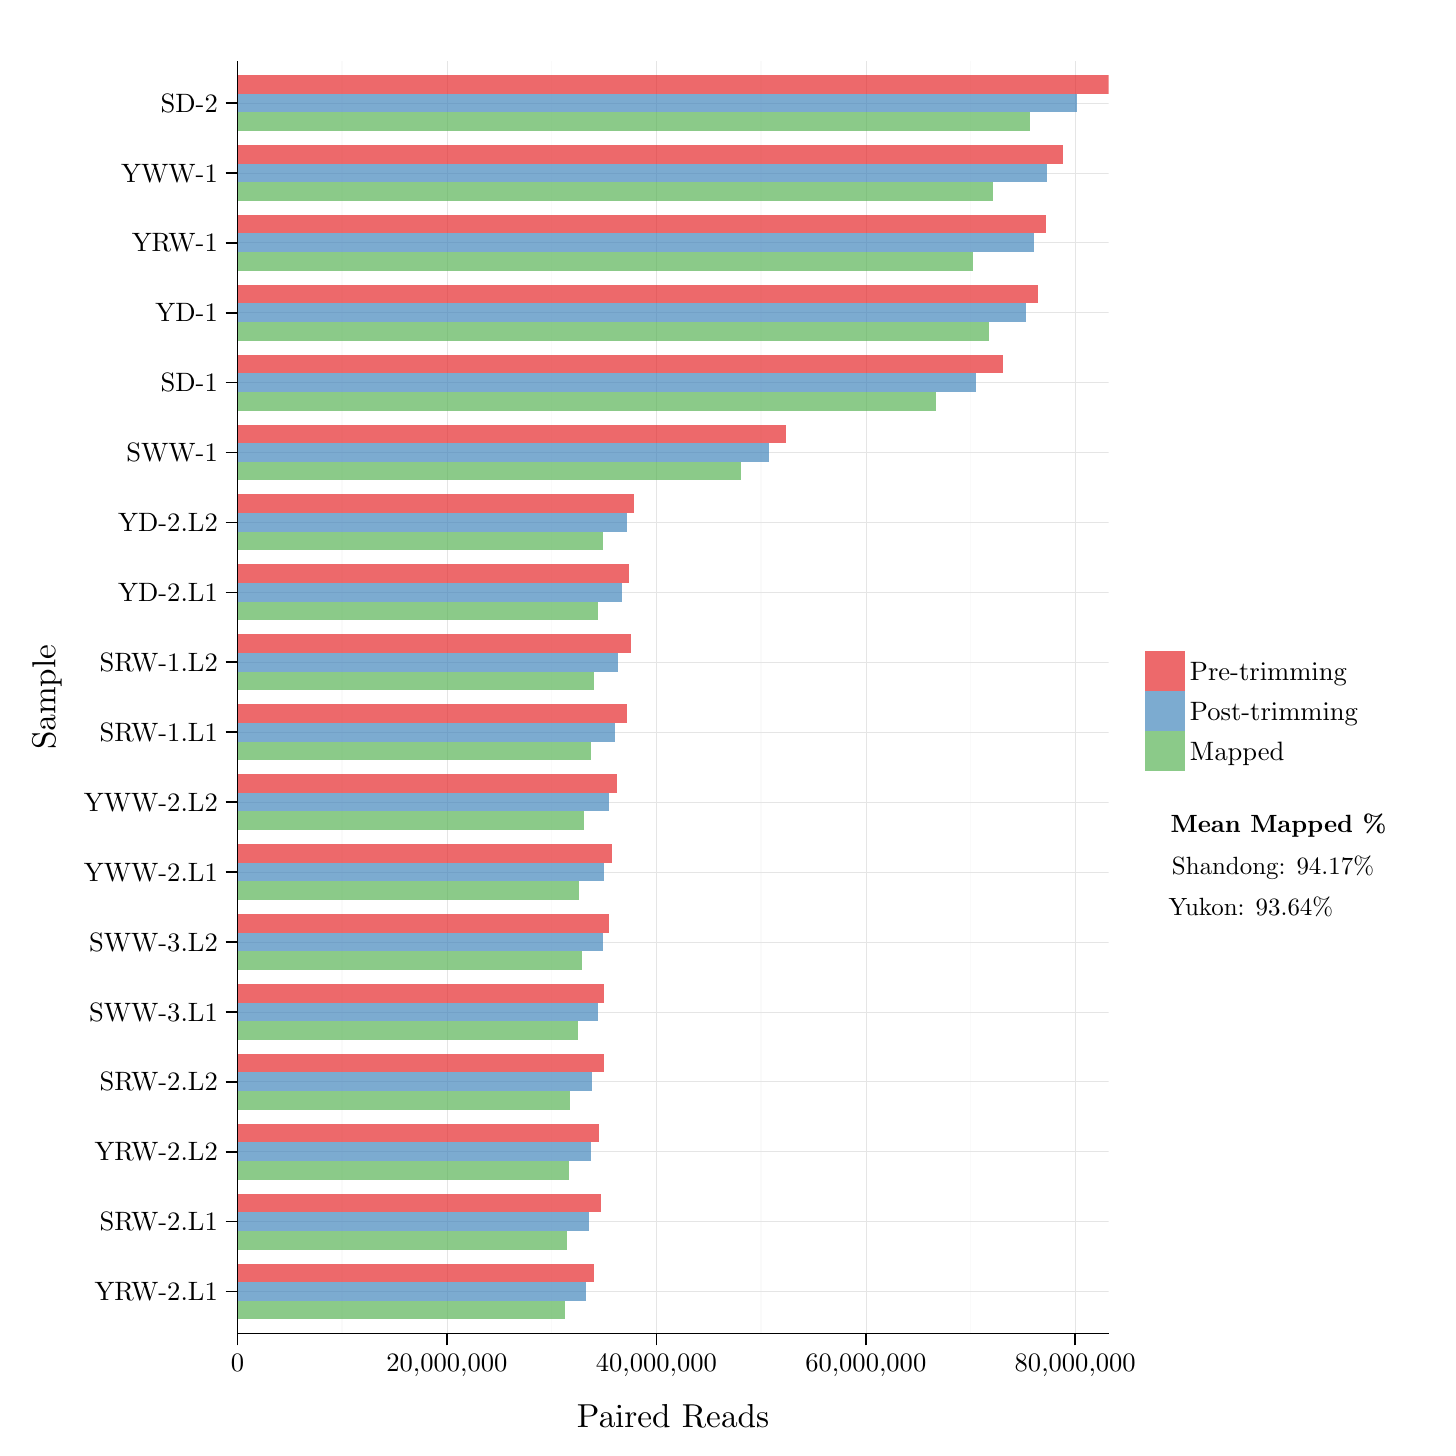
\begin{tikzpicture}[x=1pt,y=1pt]
\definecolor{fillColor}{RGB}{255,255,255}
\path[use as bounding box,fill=fillColor,fill opacity=0.00] (0,0) rectangle (505.89,505.89);
\begin{scope}
\path[clip] (  0.00,  0.00) rectangle (505.89,505.89);
\definecolor{drawColor}{RGB}{255,255,255}
\definecolor{fillColor}{RGB}{255,255,255}

\path[draw=drawColor,line width= 0.6pt,line join=round,line cap=round,fill=fillColor] (  0.00,  0.00) rectangle (505.89,505.89);
\end{scope}
\begin{scope}
\path[clip] ( 75.81, 34.03) rectangle (390.58,493.85);
\definecolor{fillColor}{RGB}{255,255,255}

\path[fill=fillColor] ( 75.81, 34.03) rectangle (390.58,493.85);
\definecolor{drawColor}{gray}{0.98}

\path[draw=drawColor,line width= 0.6pt,line join=round] (113.65, 34.03) --
	(113.65,493.85);

\path[draw=drawColor,line width= 0.6pt,line join=round] (189.33, 34.03) --
	(189.33,493.85);

\path[draw=drawColor,line width= 0.6pt,line join=round] (265.01, 34.03) --
	(265.01,493.85);

\path[draw=drawColor,line width= 0.6pt,line join=round] (340.69, 34.03) --
	(340.69,493.85);
\definecolor{drawColor}{gray}{0.90}

\path[draw=drawColor,line width= 0.2pt,line join=round] ( 75.81, 49.19) --
	(390.58, 49.19);

\path[draw=drawColor,line width= 0.2pt,line join=round] ( 75.81, 74.46) --
	(390.58, 74.46);

\path[draw=drawColor,line width= 0.2pt,line join=round] ( 75.81, 99.72) --
	(390.58, 99.72);

\path[draw=drawColor,line width= 0.2pt,line join=round] ( 75.81,124.99) --
	(390.58,124.99);

\path[draw=drawColor,line width= 0.2pt,line join=round] ( 75.81,150.25) --
	(390.58,150.25);

\path[draw=drawColor,line width= 0.2pt,line join=round] ( 75.81,175.51) --
	(390.58,175.51);

\path[draw=drawColor,line width= 0.2pt,line join=round] ( 75.81,200.78) --
	(390.58,200.78);

\path[draw=drawColor,line width= 0.2pt,line join=round] ( 75.81,226.04) --
	(390.58,226.04);

\path[draw=drawColor,line width= 0.2pt,line join=round] ( 75.81,251.31) --
	(390.58,251.31);

\path[draw=drawColor,line width= 0.2pt,line join=round] ( 75.81,276.57) --
	(390.58,276.57);

\path[draw=drawColor,line width= 0.2pt,line join=round] ( 75.81,301.84) --
	(390.58,301.84);

\path[draw=drawColor,line width= 0.2pt,line join=round] ( 75.81,327.10) --
	(390.58,327.10);

\path[draw=drawColor,line width= 0.2pt,line join=round] ( 75.81,352.36) --
	(390.58,352.36);

\path[draw=drawColor,line width= 0.2pt,line join=round] ( 75.81,377.63) --
	(390.58,377.63);

\path[draw=drawColor,line width= 0.2pt,line join=round] ( 75.81,402.89) --
	(390.58,402.89);

\path[draw=drawColor,line width= 0.2pt,line join=round] ( 75.81,428.16) --
	(390.58,428.16);

\path[draw=drawColor,line width= 0.2pt,line join=round] ( 75.81,453.42) --
	(390.58,453.42);

\path[draw=drawColor,line width= 0.2pt,line join=round] ( 75.81,478.69) --
	(390.58,478.69);

\path[draw=drawColor,line width= 0.2pt,line join=round] ( 75.81, 34.03) --
	( 75.81,493.85);

\path[draw=drawColor,line width= 0.2pt,line join=round] (151.49, 34.03) --
	(151.49,493.85);

\path[draw=drawColor,line width= 0.2pt,line join=round] (227.17, 34.03) --
	(227.17,493.85);

\path[draw=drawColor,line width= 0.2pt,line join=round] (302.85, 34.03) --
	(302.85,493.85);

\path[draw=drawColor,line width= 0.2pt,line join=round] (378.53, 34.03) --
	(378.53,493.85);
\definecolor{fillColor}{RGB}{228,26,28}

\path[fill=fillColor,fill opacity=0.65] ( 75.81, 52.56) rectangle (204.60, 59.30);
\definecolor{fillColor}{RGB}{55,126,184}

\path[fill=fillColor,fill opacity=0.65] ( 75.81, 45.82) rectangle (201.91, 52.56);
\definecolor{fillColor}{RGB}{77,175,74}

\path[fill=fillColor,fill opacity=0.65] ( 75.81, 39.09) rectangle (194.13, 45.82);
\definecolor{fillColor}{RGB}{228,26,28}

\path[fill=fillColor,fill opacity=0.65] ( 75.81, 77.83) rectangle (207.05, 84.56);
\definecolor{fillColor}{RGB}{55,126,184}

\path[fill=fillColor,fill opacity=0.65] ( 75.81, 71.09) rectangle (202.71, 77.83);
\definecolor{fillColor}{RGB}{77,175,74}

\path[fill=fillColor,fill opacity=0.65] ( 75.81, 64.35) rectangle (194.85, 71.09);
\definecolor{fillColor}{RGB}{228,26,28}

\path[fill=fillColor,fill opacity=0.65] ( 75.81,103.09) rectangle (206.30,109.83);
\definecolor{fillColor}{RGB}{55,126,184}

\path[fill=fillColor,fill opacity=0.65] ( 75.81, 96.35) rectangle (203.55,103.09);
\definecolor{fillColor}{RGB}{77,175,74}

\path[fill=fillColor,fill opacity=0.65] ( 75.81, 89.62) rectangle (195.72, 96.35);
\definecolor{fillColor}{RGB}{228,26,28}

\path[fill=fillColor,fill opacity=0.65] ( 75.81,128.35) rectangle (208.32,135.09);
\definecolor{fillColor}{RGB}{55,126,184}

\path[fill=fillColor,fill opacity=0.65] ( 75.81,121.62) rectangle (203.87,128.35);
\definecolor{fillColor}{RGB}{77,175,74}

\path[fill=fillColor,fill opacity=0.65] ( 75.81,114.88) rectangle (196.00,121.62);
\definecolor{fillColor}{RGB}{228,26,28}

\path[fill=fillColor,fill opacity=0.65] ( 75.81,153.62) rectangle (208.39,160.36);
\definecolor{fillColor}{RGB}{55,126,184}

\path[fill=fillColor,fill opacity=0.65] ( 75.81,146.88) rectangle (206.01,153.62);
\definecolor{fillColor}{RGB}{77,175,74}

\path[fill=fillColor,fill opacity=0.65] ( 75.81,140.14) rectangle (198.71,146.88);
\definecolor{fillColor}{RGB}{228,26,28}

\path[fill=fillColor,fill opacity=0.65] ( 75.81,178.88) rectangle (210.22,185.62);
\definecolor{fillColor}{RGB}{55,126,184}

\path[fill=fillColor,fill opacity=0.65] ( 75.81,172.15) rectangle (207.77,178.88);
\definecolor{fillColor}{RGB}{77,175,74}

\path[fill=fillColor,fill opacity=0.65] ( 75.81,165.41) rectangle (200.46,172.15);
\definecolor{fillColor}{RGB}{228,26,28}

\path[fill=fillColor,fill opacity=0.65] ( 75.81,204.15) rectangle (211.03,210.88);
\definecolor{fillColor}{RGB}{55,126,184}

\path[fill=fillColor,fill opacity=0.65] ( 75.81,197.41) rectangle (208.35,204.15);
\definecolor{fillColor}{RGB}{77,175,74}

\path[fill=fillColor,fill opacity=0.65] ( 75.81,190.67) rectangle (199.38,197.41);
\definecolor{fillColor}{RGB}{228,26,28}

\path[fill=fillColor,fill opacity=0.65] ( 75.81,229.41) rectangle (212.92,236.15);
\definecolor{fillColor}{RGB}{55,126,184}

\path[fill=fillColor,fill opacity=0.65] ( 75.81,222.67) rectangle (210.17,229.41);
\definecolor{fillColor}{RGB}{77,175,74}

\path[fill=fillColor,fill opacity=0.65] ( 75.81,215.94) rectangle (201.14,222.67);
\definecolor{fillColor}{RGB}{228,26,28}

\path[fill=fillColor,fill opacity=0.65] ( 75.81,254.68) rectangle (216.64,261.41);
\definecolor{fillColor}{RGB}{55,126,184}

\path[fill=fillColor,fill opacity=0.65] ( 75.81,247.94) rectangle (212.28,254.68);
\definecolor{fillColor}{RGB}{77,175,74}

\path[fill=fillColor,fill opacity=0.65] ( 75.81,241.20) rectangle (203.65,247.94);
\definecolor{fillColor}{RGB}{228,26,28}

\path[fill=fillColor,fill opacity=0.65] ( 75.81,279.94) rectangle (217.84,286.68);
\definecolor{fillColor}{RGB}{55,126,184}

\path[fill=fillColor,fill opacity=0.65] ( 75.81,273.20) rectangle (213.38,279.94);
\definecolor{fillColor}{RGB}{77,175,74}

\path[fill=fillColor,fill opacity=0.65] ( 75.81,266.47) rectangle (204.75,273.20);
\definecolor{fillColor}{RGB}{228,26,28}

\path[fill=fillColor,fill opacity=0.65] ( 75.81,305.20) rectangle (217.17,311.94);
\definecolor{fillColor}{RGB}{55,126,184}

\path[fill=fillColor,fill opacity=0.65] ( 75.81,298.47) rectangle (214.80,305.20);
\definecolor{fillColor}{RGB}{77,175,74}

\path[fill=fillColor,fill opacity=0.65] ( 75.81,291.73) rectangle (206.09,298.47);
\definecolor{fillColor}{RGB}{228,26,28}

\path[fill=fillColor,fill opacity=0.65] ( 75.81,330.47) rectangle (219.12,337.21);
\definecolor{fillColor}{RGB}{55,126,184}

\path[fill=fillColor,fill opacity=0.65] ( 75.81,323.73) rectangle (216.68,330.47);
\definecolor{fillColor}{RGB}{77,175,74}

\path[fill=fillColor,fill opacity=0.65] ( 75.81,316.99) rectangle (207.93,323.73);
\definecolor{fillColor}{RGB}{228,26,28}

\path[fill=fillColor,fill opacity=0.65] ( 75.81,355.73) rectangle (273.87,362.47);
\definecolor{fillColor}{RGB}{55,126,184}

\path[fill=fillColor,fill opacity=0.65] ( 75.81,349.00) rectangle (268.04,355.73);
\definecolor{fillColor}{RGB}{77,175,74}

\path[fill=fillColor,fill opacity=0.65] ( 75.81,342.26) rectangle (257.74,349.00);
\definecolor{fillColor}{RGB}{228,26,28}

\path[fill=fillColor,fill opacity=0.65] ( 75.81,381.00) rectangle (352.57,387.73);
\definecolor{fillColor}{RGB}{55,126,184}

\path[fill=fillColor,fill opacity=0.65] ( 75.81,374.26) rectangle (342.64,381.00);
\definecolor{fillColor}{RGB}{77,175,74}

\path[fill=fillColor,fill opacity=0.65] ( 75.81,367.52) rectangle (328.06,374.26);
\definecolor{fillColor}{RGB}{228,26,28}

\path[fill=fillColor,fill opacity=0.65] ( 75.81,406.26) rectangle (364.93,413.00);
\definecolor{fillColor}{RGB}{55,126,184}

\path[fill=fillColor,fill opacity=0.65] ( 75.81,399.52) rectangle (360.81,406.26);
\definecolor{fillColor}{RGB}{77,175,74}

\path[fill=fillColor,fill opacity=0.65] ( 75.81,392.79) rectangle (347.46,399.52);
\definecolor{fillColor}{RGB}{228,26,28}

\path[fill=fillColor,fill opacity=0.65] ( 75.81,431.53) rectangle (367.82,438.26);
\definecolor{fillColor}{RGB}{55,126,184}

\path[fill=fillColor,fill opacity=0.65] ( 75.81,424.79) rectangle (363.80,431.53);
\definecolor{fillColor}{RGB}{77,175,74}

\path[fill=fillColor,fill opacity=0.65] ( 75.81,418.05) rectangle (341.75,424.79);
\definecolor{fillColor}{RGB}{228,26,28}

\path[fill=fillColor,fill opacity=0.65] ( 75.81,456.79) rectangle (374.26,463.53);
\definecolor{fillColor}{RGB}{55,126,184}

\path[fill=fillColor,fill opacity=0.65] ( 75.81,450.05) rectangle (368.17,456.79);
\definecolor{fillColor}{RGB}{77,175,74}

\path[fill=fillColor,fill opacity=0.65] ( 75.81,443.32) rectangle (348.70,450.05);
\definecolor{fillColor}{RGB}{228,26,28}

\path[fill=fillColor,fill opacity=0.65] ( 75.81,482.05) rectangle (390.58,488.79);
\definecolor{fillColor}{RGB}{55,126,184}

\path[fill=fillColor,fill opacity=0.65] ( 75.81,475.32) rectangle (378.99,482.05);
\definecolor{fillColor}{RGB}{77,175,74}

\path[fill=fillColor,fill opacity=0.65] ( 75.81,468.58) rectangle (362.15,475.32);
\end{scope}
\begin{scope}
\path[clip] (  0.00,  0.00) rectangle (505.89,505.89);
\definecolor{drawColor}{RGB}{0,0,0}

\path[draw=drawColor,line width= 0.6pt,line join=round] ( 75.81, 34.03) --
	( 75.81,493.85);
\end{scope}
\begin{scope}
\path[clip] (  0.00,  0.00) rectangle (505.89,505.89);
\definecolor{drawColor}{RGB}{0,0,0}

\node[text=drawColor,anchor=base east,inner sep=0pt, outer sep=0pt, scale=  0.96] at ( 68.70, 45.89) {YRW-2.L1};

\node[text=drawColor,anchor=base east,inner sep=0pt, outer sep=0pt, scale=  0.96] at ( 68.70, 71.15) {SRW-2.L1};

\node[text=drawColor,anchor=base east,inner sep=0pt, outer sep=0pt, scale=  0.96] at ( 68.70, 96.42) {YRW-2.L2};

\node[text=drawColor,anchor=base east,inner sep=0pt, outer sep=0pt, scale=  0.96] at ( 68.70,121.68) {SRW-2.L2};

\node[text=drawColor,anchor=base east,inner sep=0pt, outer sep=0pt, scale=  0.96] at ( 68.70,146.94) {SWW-3.L1};

\node[text=drawColor,anchor=base east,inner sep=0pt, outer sep=0pt, scale=  0.96] at ( 68.70,172.21) {SWW-3.L2};

\node[text=drawColor,anchor=base east,inner sep=0pt, outer sep=0pt, scale=  0.96] at ( 68.70,197.47) {YWW-2.L1};

\node[text=drawColor,anchor=base east,inner sep=0pt, outer sep=0pt, scale=  0.96] at ( 68.70,222.74) {YWW-2.L2};

\node[text=drawColor,anchor=base east,inner sep=0pt, outer sep=0pt, scale=  0.96] at ( 68.70,248.00) {SRW-1.L1};

\node[text=drawColor,anchor=base east,inner sep=0pt, outer sep=0pt, scale=  0.96] at ( 68.70,273.27) {SRW-1.L2};

\node[text=drawColor,anchor=base east,inner sep=0pt, outer sep=0pt, scale=  0.96] at ( 68.70,298.53) {YD-2.L1};

\node[text=drawColor,anchor=base east,inner sep=0pt, outer sep=0pt, scale=  0.96] at ( 68.70,323.79) {YD-2.L2};

\node[text=drawColor,anchor=base east,inner sep=0pt, outer sep=0pt, scale=  0.96] at ( 68.70,349.06) {SWW-1};

\node[text=drawColor,anchor=base east,inner sep=0pt, outer sep=0pt, scale=  0.96] at ( 68.70,374.32) {SD-1};

\node[text=drawColor,anchor=base east,inner sep=0pt, outer sep=0pt, scale=  0.96] at ( 68.70,399.59) {YD-1};

\node[text=drawColor,anchor=base east,inner sep=0pt, outer sep=0pt, scale=  0.96] at ( 68.70,424.85) {YRW-1};

\node[text=drawColor,anchor=base east,inner sep=0pt, outer sep=0pt, scale=  0.96] at ( 68.70,450.12) {YWW-1};

\node[text=drawColor,anchor=base east,inner sep=0pt, outer sep=0pt, scale=  0.96] at ( 68.70,475.38) {SD-2};
\end{scope}
\begin{scope}
\path[clip] (  0.00,  0.00) rectangle (505.89,505.89);
\definecolor{drawColor}{RGB}{0,0,0}

\path[draw=drawColor,line width= 0.6pt,line join=round] ( 71.54, 49.19) --
	( 75.81, 49.19);

\path[draw=drawColor,line width= 0.6pt,line join=round] ( 71.54, 74.46) --
	( 75.81, 74.46);

\path[draw=drawColor,line width= 0.6pt,line join=round] ( 71.54, 99.72) --
	( 75.81, 99.72);

\path[draw=drawColor,line width= 0.6pt,line join=round] ( 71.54,124.99) --
	( 75.81,124.99);

\path[draw=drawColor,line width= 0.6pt,line join=round] ( 71.54,150.25) --
	( 75.81,150.25);

\path[draw=drawColor,line width= 0.6pt,line join=round] ( 71.54,175.51) --
	( 75.81,175.51);

\path[draw=drawColor,line width= 0.6pt,line join=round] ( 71.54,200.78) --
	( 75.81,200.78);

\path[draw=drawColor,line width= 0.6pt,line join=round] ( 71.54,226.04) --
	( 75.81,226.04);

\path[draw=drawColor,line width= 0.6pt,line join=round] ( 71.54,251.31) --
	( 75.81,251.31);

\path[draw=drawColor,line width= 0.6pt,line join=round] ( 71.54,276.57) --
	( 75.81,276.57);

\path[draw=drawColor,line width= 0.6pt,line join=round] ( 71.54,301.84) --
	( 75.81,301.84);

\path[draw=drawColor,line width= 0.6pt,line join=round] ( 71.54,327.10) --
	( 75.81,327.10);

\path[draw=drawColor,line width= 0.6pt,line join=round] ( 71.54,352.36) --
	( 75.81,352.36);

\path[draw=drawColor,line width= 0.6pt,line join=round] ( 71.54,377.63) --
	( 75.81,377.63);

\path[draw=drawColor,line width= 0.6pt,line join=round] ( 71.54,402.89) --
	( 75.81,402.89);

\path[draw=drawColor,line width= 0.6pt,line join=round] ( 71.54,428.16) --
	( 75.81,428.16);

\path[draw=drawColor,line width= 0.6pt,line join=round] ( 71.54,453.42) --
	( 75.81,453.42);

\path[draw=drawColor,line width= 0.6pt,line join=round] ( 71.54,478.69) --
	( 75.81,478.69);
\end{scope}
\begin{scope}
\path[clip] (  0.00,  0.00) rectangle (505.89,505.89);
\definecolor{drawColor}{RGB}{0,0,0}

\path[draw=drawColor,line width= 0.6pt,line join=round] ( 75.81, 34.03) --
	(390.58, 34.03);
\end{scope}
\begin{scope}
\path[clip] (  0.00,  0.00) rectangle (505.89,505.89);
\definecolor{drawColor}{RGB}{0,0,0}

\path[draw=drawColor,line width= 0.6pt,line join=round] ( 75.81, 29.77) --
	( 75.81, 34.03);

\path[draw=drawColor,line width= 0.6pt,line join=round] (151.49, 29.77) --
	(151.49, 34.03);

\path[draw=drawColor,line width= 0.6pt,line join=round] (227.17, 29.77) --
	(227.17, 34.03);

\path[draw=drawColor,line width= 0.6pt,line join=round] (302.85, 29.77) --
	(302.85, 34.03);

\path[draw=drawColor,line width= 0.6pt,line join=round] (378.53, 29.77) --
	(378.53, 34.03);
\end{scope}
\begin{scope}
\path[clip] (  0.00,  0.00) rectangle (505.89,505.89);
\definecolor{drawColor}{RGB}{0,0,0}

\node[text=drawColor,anchor=base,inner sep=0pt, outer sep=0pt, scale=  0.96] at ( 75.81, 20.31) {0};

\node[text=drawColor,anchor=base,inner sep=0pt, outer sep=0pt, scale=  0.96] at (151.49, 20.31) {20,000,000};

\node[text=drawColor,anchor=base,inner sep=0pt, outer sep=0pt, scale=  0.96] at (227.17, 20.31) {40,000,000};

\node[text=drawColor,anchor=base,inner sep=0pt, outer sep=0pt, scale=  0.96] at (302.85, 20.31) {60,000,000};

\node[text=drawColor,anchor=base,inner sep=0pt, outer sep=0pt, scale=  0.96] at (378.53, 20.31) {80,000,000};
\end{scope}
\begin{scope}
\path[clip] (  0.00,  0.00) rectangle (505.89,505.89);
\definecolor{drawColor}{RGB}{0,0,0}

\node[text=drawColor,anchor=base,inner sep=0pt, outer sep=0pt, scale=  1.20] at (233.20,  0) {Paired Reads};
\end{scope}
\begin{scope}
\path[clip] (  0.00,  0.00) rectangle (505.89,505.89);
\definecolor{drawColor}{RGB}{0,0,0}

\node[text=drawColor,rotate= 90.00,anchor=base,inner sep=0pt, outer sep=0pt, scale=  1.20] at ( 10,263.94) {Sample};
\end{scope}
\begin{scope}
\path[clip] (  0.00,  0.00) rectangle (505.89,505.89);
\definecolor{fillColor}{RGB}{255,255,255}

\path[fill=fillColor] (399.45,232.87) rectangle (484.98,295.01);
\end{scope}
\begin{scope}
\path[clip] (  0.00,  0.00) rectangle (505.89,505.89);
\definecolor{drawColor}{gray}{0.80}
\definecolor{fillColor}{RGB}{255,255,255}

\begin{scope}
\path[clip] (  0.00,  0.00) rectangle (505.89,505.89);
\definecolor{drawColor}{RGB}{0,0,0}

\node[text=drawColor,font=\bf,rotate= 0,anchor=base,inner sep=0pt, outer sep=0pt, scale=  0.90] at ( 452,215) {Mean Mapped \%};
\end{scope}
\begin{scope}
\path[clip] (  0.00,  0.00) rectangle (505.89,505.89);
\definecolor{drawColor}{RGB}{0,0,0}

\node[text=drawColor,rotate= 0,anchor=base,inner sep=0pt, outer sep=0pt, scale=  0.90] at ( 450,200) {Shandong: 94.17\%};
\end{scope}
\begin{scope}
\path[clip] (  0.00,  0.00) rectangle (505.89,505.89);
\definecolor{drawColor}{RGB}{0,0,0}

\node[text=drawColor,rotate= 0,anchor=base,inner sep=0pt, outer sep=0pt, scale=  0.90] at ( 442,185) {Yukon: 93.64\%};
\end{scope}
%\path[draw=drawColor,line width= 0.6pt,line join=round,line cap=round,fill=fillColor] (403.72,266.05) rectangle (418.17,280.50);
\end{scope}
\begin{scope}
\path[clip] (  0.00,  0.00) rectangle (505.89,505.89);
\definecolor{fillColor}{RGB}{77,175,74}

%green
\path[fill=fillColor,fill opacity=0.65] (403.72,237.14) rectangle (418.17,251.59);

\path[] (403.72,266.05) --
	(418.17,280.50);
\end{scope}
\begin{scope}
\path[clip] (  0.00,  0.00) rectangle (505.89,505.89);
\definecolor{drawColor}{gray}{0.80}
\definecolor{fillColor}{RGB}{255,255,255}

%\path[draw=drawColor,line width= 0.6pt,line join=round,line cap=round,fill=fillColor] (403.72,251.59) rectangle (418.17,266.05);
\end{scope}
\begin{scope}
\path[clip] (  0.00,  0.00) rectangle (505.89,505.89);
\definecolor{fillColor}{RGB}{55,126,184}

%blue
\path[fill=fillColor,fill opacity=0.65] (403.72,251.59) rectangle (418.17,266.05);

\path[] (403.72,251.59) --
	(418.17,266.05);
\end{scope}
\begin{scope}
\path[clip] (  0.00,  0.00) rectangle (505.89,505.89);
\definecolor{drawColor}{gray}{0.80}
\definecolor{fillColor}{RGB}{255,255,255}

%\path[draw=drawColor,line width= 0.6pt,line join=round,line cap=round,fill=fillColor] (403.72,237.14) rectangle (418.17,251.59);
\end{scope}
\begin{scope}
\path[clip] (  0.00,  0.00) rectangle (505.89,505.89);
\definecolor{fillColor}{RGB}{228,26,28}

%red
\path[fill=fillColor,fill opacity=0.65] (403.72,266.05) rectangle (418.17,280.50);

\path[] (403.72,237.14) --
	(418.17,251.59);
\end{scope}
\begin{scope}
\path[clip] (  0.00,  0.00) rectangle (505.89,505.89);
\definecolor{drawColor}{RGB}{0,0,0}

\node[text=drawColor,anchor=base west,inner sep=0pt, outer sep=0pt, scale=  0.96] at (419.98,241.06) {Mapped};
\end{scope}
\begin{scope}
\path[clip] (  0.00,  0.00) rectangle (505.89,505.89);
\definecolor{drawColor}{RGB}{0,0,0}

\node[text=drawColor,anchor=base west,inner sep=0pt, outer sep=0pt, scale=  0.96] at (419.98,255.51) {Post-trimming};
\end{scope}
\begin{scope}
\path[clip] (  0.00,  0.00) rectangle (505.89,505.89);
\definecolor{drawColor}{RGB}{0,0,0}

\node[text=drawColor,anchor=base west,inner sep=0pt, outer sep=0pt, scale=  0.96] at (419.98,269.97) {Pre-trimming};
\end{scope}
\end{tikzpicture}
